\section{Технический проект}
\subsection{Общие сведения о программной системе}

Необходимо спроектировать и разработать веб-приложение для освещения инцидентов, связанных с общественным транспортом, такими как автобусы, троллейбусы и маршрутные такси. Это веб-приложение предоставит пользователям возможность просматривать посты и видеозаписи, содержащие информацию об инцидентах с общественным транспортом.

Для доступа к просмотру или оставлению обращений пользователи должны будут зарегистрироваться или войти в систему. Это обеспечит контроль над контентом и позволит отслеживать активность каждого пользователя. Пользователи смогут оставлять свои обращения о случившихся инцидентах, заполняя форму обратной связи, где они будут описывать произошедшее событие. Зарегистрированные пользователи смогут просматривать все доступные посты и видеозаписи, связанные с инцидентами, которые будут отображаться в формате новостной ленты. Все оставленные обращения будут проходить обязательную модерацию, в ходе которой тексты будут проверяться на отсутствие неподобающего контента. Только обращения, прошедшие модерацию, будут публиковаться в ленте.

Администраторы получат расширенные права доступа, позволяющие им добавлять новых водителей в базу данных, редактировать существующую информацию, а также управлять обращениями. Административная панель предоставит все необходимые инструменты для выполнения этих задач. В приложении будет предусмотрена функция отображения рейтинга водителей, что позволит пассажирам оценивать их работу и оставлять обратную связь. Пользователи также будут иметь доступ к личному кабинету, где они смогут управлять своей информацией, просматривать свои обращения и взаимодействовать с приложением.

Это веб-приложение предназначено для освещения инцидентов, связанных с общественным городским транспортом, и будет служить платформой для обмена информацией между пассажирами и ответственными органами. Основная цель системы — предоставлять актуальные данные о происшествиях, чтобы ответственные службы могли оперативно реагировать на возникающие проблемы и улучшать качество обслуживания общественного транспорта.

\subsection{Проектирование архитектуры программной системы}

\subsubsection{Выбор архитектурного стиля и паттернов проектирования}

Архитектурный стиль и паттерны проектирования имеют ключевое значение при создании высокопроизводительных, масштабируемых и безопасных систем, особенно в контексте разработки REST API. REST API (Representational State Transfer Application Programming Interface) представляет собой архитектурный подход, который основывается на принципах унифицированных интерфейсов и передачи состояния между клиентом и сервером. В процессе разработки REST API критически важно выбрать правильный архитектурный стиль и использовать соответствующие паттерны проектирования, чтобы обеспечить эффективную работу системы и удовлетворение требований пользователей.

Клиент-серверная архитектура является одним из фундаментальных аспектов разработки REST API. Этот архитектурный стиль разделяет систему на две основные части: клиентскую, которая отправляет запросы на сервер, и серверную, которая обрабатывает эти запросы и возвращает результаты. Такая структура позволяет создавать масштабируемые и гибкие системы, способные обрабатывать большие объемы запросов от множества клиентов одновременно.

Одним из важных паттернов проектирования для REST API является паттерн Facade, который позволяет создать единый интерфейс для взаимодействия с комплексной системой, скрывая сложные детали реализации и предоставляя простой и интуитивно понятный интерфейс для пользователей. Использование паттерна Facade повышает модульность и гибкость REST API, облегчая его использование и сопровождение.

Также значимым паттерном является Адаптер. В контексте REST API, паттерн Адаптер позволяет преобразовывать данные из одного формата в другой, что обеспечивает совместимость между различными системами и источниками данных. Например, если данные поступают в формате, который необходимо преобразовать для работы с REST API, Адаптер справляется с этой задачей, гарантируя единообразие данных в системе.

Для обеспечения безопасности данных в REST API широко используются протокол HTTPS и технология ODBC (Open Database Connectivity). Протокол HTTPS обеспечивает защищенное соединение между клиентом и сервером, шифруя данные и предотвращая их несанкционированный доступ или изменение. Технология ODBC предоставляет универсальный интерфейс для взаимодействия с различными базами данных, обеспечивая безопасную и эффективную работу с данными в REST API.

Архитектура системы представлена на рисунке ~\ref{templ:image12}.
\begin{figure}[H]
	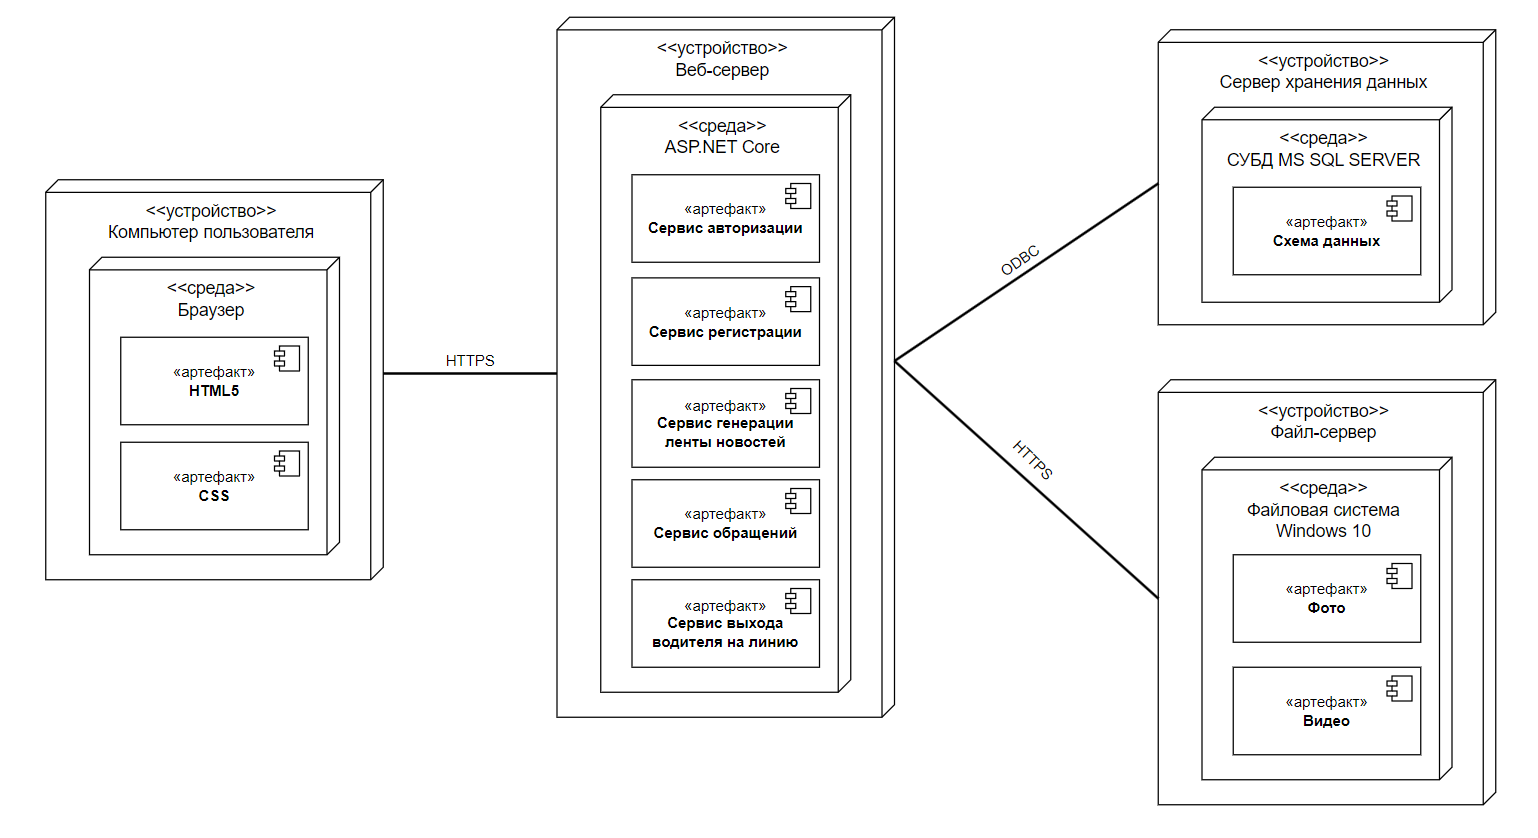
\includegraphics[width=1\linewidth]{Архитектура программной системы}
	\caption{Архитектура программной системы}
	\label{templ:image12}
\end{figure}

\subsubsection{Описание REST API микросервисов}

\begin{xltabular}{\textwidth}{|X|X|X|X|}
	\caption{Описание методов для работы с новостной лентой}\label{prod:table35}\\\hline HTTP-метод & Описание & Входные параметры & Выходные параметры \\ \hline
	\endfirsthead
	\caption[]{Продолжение таблицы \ref{prod:table35}}\\\hline 
	HTTP-метод & Описание & Входные параметры & Выходные параметры \\ \hline
	\endhead
	GET /api/News
	Generator
	Controller & Получение всех записей из таблицы & - & Ratings: List<object> \\ \hline
	GET /api/ Employee
	GET /api/News
	Generator
	Controller/:id & Получение конкретной записи из таблицы & RatingId: integer & Rating: object \\ \hline
	GET /api/News
	Generator
	Controller
	/noPublished & Получение записей, которые еще не были опубликованы & PublishedEntry: bool & Ratings: List<object> \\ \hline
	POST /api/News
	Generator
	Controllerd & Добавление новой записи & Data: object & Rating: object \\ \hline
	PUT /api/News
	Generator
	Controller/:id & Обновление записи в таблице & RatingId: integer,
	RatingUp: object & Rating: object \\ \hline
	DELETE /api/News
	Generator
	Controller/:id & Удаление записи из таблицы & RatingId: integer & - \\ \hline
\end{xltabular}

\begin{xltabular}{\textwidth}{|X|X|X|X|}
	\caption{Описание методов для работы авторизации и регистрации}\label{prod:table36}\\\hline 
	HTTP-метод & Описание & Входные параметры & Выходные параметры \\ \hline
	\endfirsthead
	\caption[]{Продолжение таблицы \ref{prod:table36}}\\\hline 
	HTTP-метод & Описание & Входные параметры & Выходные параметры \\ \hline
	\endhead
	POST /api/
	Autorisation
	Controller/
	registration & Регистрация нового пассажира & Data: object & Passenger: object \\ \hline
	POST /api/
	Autorisation
	Controller/:
	login & Авторизация пользователя & Login: string, Password: string & UserId: integer, RoleInTheSystem: string \\ \hline
\end{xltabular}

\begin{xltabular}{\textwidth}{|X|X|X|X|}
	\caption{Описание методов для работы с маршрутами}\label{prod:table37}\\\hline 
	HTTP-метод & Описание & Входные параметры & Выходные параметры \\ \hline
	\endfirsthead
	\caption[]{Продолжение таблицы \ref{prod:table37}}\\\hline 
	HTTP-метод & Описание & Входные параметры & Выходные параметры \\ \hline
	\endhead
	POST /api/
	UrbanRoute
	Controller & Добавление нового маршрута & Data: object & UrbanRoute: object \\ \hline
	GET /api/ 
	UrbanRoute
	Controller/:id & Получение нужного маршрута & RouteId: integer & UrbanRoute: object \\ \hline
	GET /api/
	UrbanRoute
	Controller & Получение всех маршрутов & - & UrbanRoutes: List<object> \\ \hline
	PUT /api/ 
	UrbanRoute
	Controller/:id & Обновление данных о маршруте & RouteId: integer, UrbanRouteUp: object & UrbanRoute: object \\ \hline
	DELETE /api/
	UrbanRoute
	Controller/:id & Удаление маршрута & RouteId: integer & - \\ \hline
\end{xltabular}

\begin{xltabular}{\textwidth}{|X|X|X|X|}
	\caption{Описание методов для работы с водителями}\label{prod:table32}\\\hline HTTP-метод & Описание & Входные параметры & Выходные параметры \\ \hline
	\endfirsthead
	\caption[]{Продолжение таблицы \ref{prod:table32}}\\\hline 
	HTTP-метод & Описание & Входные параметры & Выходные параметры \\ \hline
	\endhead
	POST /api/Driver
	Controller & Добавление данных о водителе & Data: object & Driver: object \\ \hline
	GET /api/Driver
	Controller/:id & Получение данных о водителе & UserId: integer & Driver: object \\ \hline
	PUT /api/Driver
	Controller/:id & Обновление данных водителя & UserId: integer, DriverUp: object & Driver: object \\ \hline
	DELETE /api/Driver
	Controller/:id & Удаление данных о водителе & UserId: integer & - \\ \hline
\end{xltabular}

\begin{xltabular}{\textwidth}{|X|X|X|X|}
	\caption{Описание методов для работы с пассажирами}\label{prod:table33}\\\hline HTTP-метод & Описание & Входные параметры & Выходные параметры \\ \hline
	\endfirsthead
	\caption[]{Продолжение таблицы \ref{prod:table33}}\\\hline 
	HTTP-метод & Описание & Входные параметры & Выходные параметры \\ \hline
	\endhead
	GET /api/Passenger
	Controller/:id & Получение данных о пассажире & UserId: integer & Passenger: object \\ \hline
	PUT /api/Passenger
	Controller/:idd & Обновление данных пассажира & UserId: integer, PassengerUp: object & Passenger: object \\ \hline
	DELETE /api/Passenger
	Controller/:id & Удаление данных о пассажире & UserId: integer & - \\ \hline
\end{xltabular}

\begin{xltabular}{\textwidth}{|X|X|X|X|}
	\caption{Описание методов для работы с сотрудниками}\label{prod:table34}\\\hline HTTP-метод & Описание & Входные параметры & Выходные параметры \\ \hline
	\endfirsthead
	\caption[]{Продолжение таблицы \ref{prod:table34♦}}\\\hline 
	HTTP-метод & Описание & Входные параметры & Выходные параметры \\ \hline
	\endhead
	POST /api/ Employee
	Controller & Добавление нового сотрудника & Data: object & Employee: object \\ \hline
	GET /api/ Employee
	Controller/:id & Получение данных о сотруднике & UserId: integer & Employee: object \\ \hline
	PUT /api/ Employee
	Controller/:id & Обновление данных сотрудника & UserId: integer, EmployeeUp: object & Employee: object \\ \hline
	DELETE /api/ 
	Employee
	Controller/:id & Удаление данных о сотруднике & UserId: integer & - \\ \hline
\end{xltabular}

\subsubsection{Структура базы данных}

В качестве системы управления базами данных была выбрана реляционная СУБД Microsoft SQL Server. Она предназначена для хранения и управления данными, а также для выполнения различных задач по их обработке, анализу и управлению. SQL Server используется в корпоративных приложениях, веб-приложениях и других системах, где требуется надежное и масштабируемое хранилище данных.

Microsoft SQL Server обладает рядом преимуществ, которые делают его оптимальным выбором для управления базами данных в различных проектах. К ключевым преимуществам можно отнести:
\begin{itemize}
	\item Высокая производительность. SQL Server оптимизирован для высокой производительности как для транзакционных рабочих нагрузок, так и для аналитических запросов. Он включает в себя технологии, такие как in-memory processing и параллельное выполнение запросов, что позволяет обрабатывать большие объемы данных эффективно.
	\item Безопасность данных. SQL Server предоставляет обширные возможности для обеспечения безопасности данных. В него встроены функции шифрования данных, аутентификации, управления доступом на основе ролей (RBAC), а также средства для аудита и мониторинга безопасности.
	\item Высокая доступность и отказоустойчивость. Существует несколько функций для обеспечения высокой доступности и отказоустойчивости, включая Always On Availability Groups, репликацию и зеркалирование баз данных. Эти функции помогают минимизировать время простоя и обеспечивают непрерывный доступ к данным.
	\item Масштабируемость. SQL Server может масштабироваться как вертикально, так и горизонтально. Он поддерживает работу на разных уровнях — от небольших приложений до крупных корпоративных систем с большими объемами данных и высокой нагрузкой.
	\item Обширная поддержка и документация. Microsoft предоставляет обширную документацию, поддержку и ресурсы для обучения. Это включает в себя онлайн-документацию, форумы, обучающие курсы и официальные сертификации, что помогает администраторам и разработчикам быстро освоить и эффективно использовать SQL Server.
\end{itemize}

Несмотря на многочисленные преимущества, Microsoft SQL Server имеет и некоторые недостатки, которые могут быть значимыми в зависимости от конкретных требований и условий эксплуатации. К недостаткам можно отнести:
\begin{itemize}
	\item Обновления и совместимость. Обновления SQL Server могут вызывать затруднения и иногда могут создавать проблемы с совместимостью приложений, особенно если они зависят от определенных версий или функций базы данных. Это требует тщательного планирования и тестирования перед внедрением обновлений.
	\item Ограниченная кроссплатформенность. Хотя в последние годы Microsoft сделала шаги в сторону кроссплатформенности (например, выпустила версии SQL Server для Linux), основная платформа и многие функции SQL Server всё ещё оптимизированы для работы на Windows. 
	\item Требования к аппаратному обеспечению. Для достижения максимальной производительности SQL Server требует значительных ресурсов аппаратного обеспечения, таких как процессор, память и дисковое пространство.
\end{itemize}

\paragraph{Схема данных}

На основании анализа предметной области и технического задания была разработана база данных, предназначенная для хранения и обработки хранящейся информации. Схема данных представлена на рисунке ~\ref{templ:image1}.
\begin{figure}[H]
	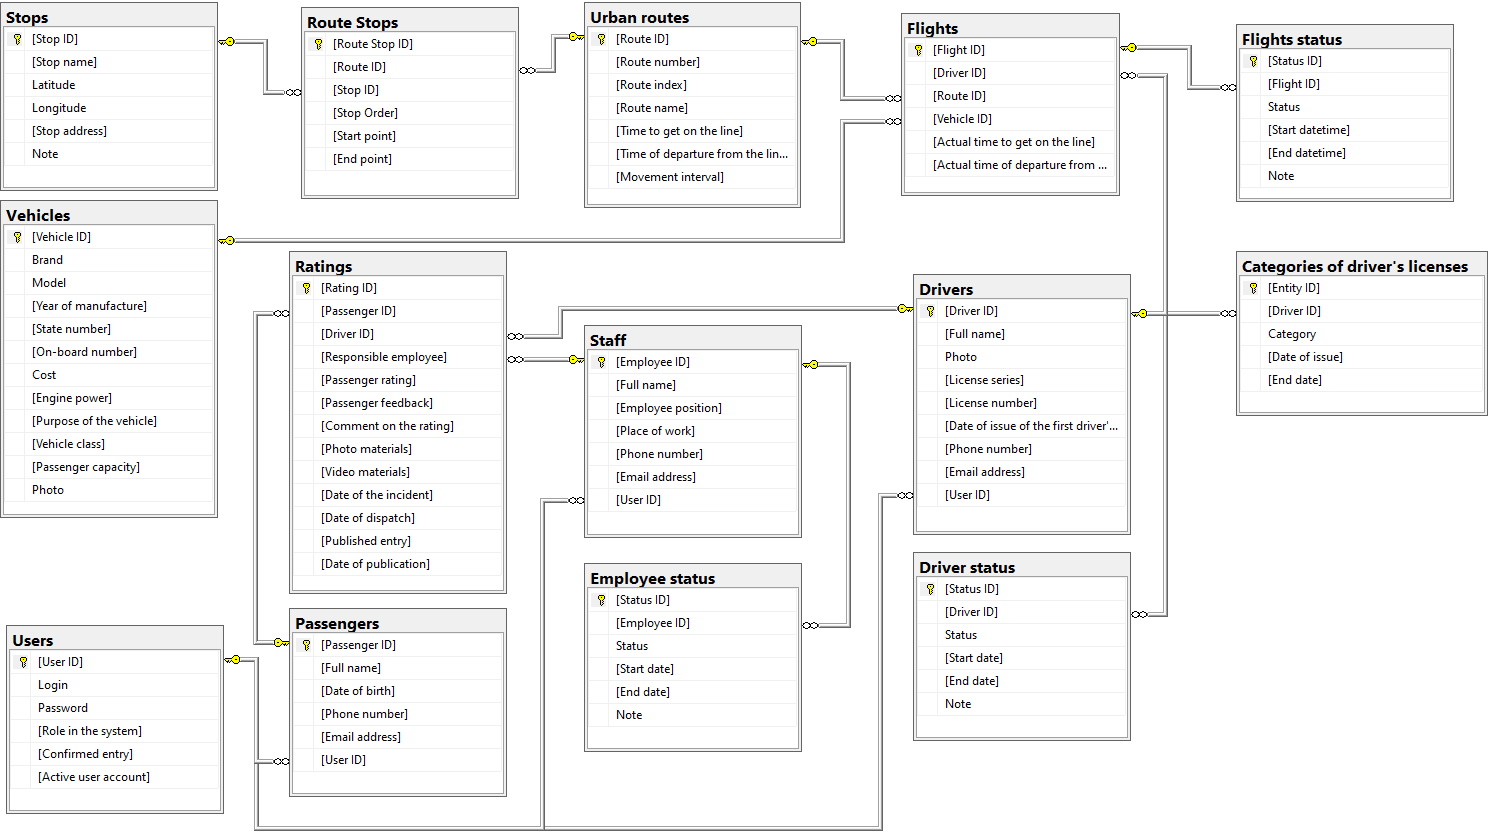
\includegraphics[width=1\linewidth]{Схема данных}
	\caption{Схема данных}
	\label{templ:image1}
\end{figure}

Все сущности базы данных приведены к третьей нормальной форме, что означает, что каждая таблица удовлетворяет требованиям нормализации:
\begin{enumerate}
	\item Отсутствие дублирования данных. В каждой таблице данные не дублируются, что помогает избежать избыточности и обеспечивает экономное использование ресурсов.
	\item Зависимость атрибутов от первичного ключа. Все неключевые атрибуты в таблице зависят только от первичного ключа, а не от других неключевых атрибутов. Это гарантирует, что каждая таблица содержит данные, относящиеся к одному логическому объекту или концепции.
	\item Устранение транзитивных зависимостей. Если атрибуты зависят друг от друга через другой атрибут, такие зависимости устранены. Это обеспечивает целостность данных и упрощает процесс обновления и удаления данных.
\end{enumerate}

\paragraph{Описание схемы данных}

Ниже приведено полное описание структуры базы данных, включая все таблицы и их атрибуты.

\begin{xltabular}{\textwidth}{|c|X|X|X|X|X|}
	\caption{Описание таблицы "<Users">\label{prod:table1}}\\ \hline
	\centrow Key Type & \centrow Optionality & \centrow Column Name & \centrow Data Type & \centrow Size \\ \hline
	\centrow pk & \centrow * & \thead{User ID} & \centrow INTEGER & \\ \hline
	\endfirsthead
	\continuecaption{Продолжение таблицы \ref{prod:table1}}
	\centrow Key Type & \centrow Optionality & \centrow Column Name & \centrow Data Type & \centrow Size \\ \hline
	\finishhead
	& \centrow * & \centrow Login & \centrow NVARCHAR & \centrow 100 \\ \hline 
	& \centrow * & \centrow Password & \centrow NVARCHAR & \centrow 100 \\ \hline
	& \centrow * & \centrow Role in the system & \centrow NVARCHAR & \centrow 15 \\ \hline 
	& \centrow ° & \centrow Confirmed entry & \centrow BIT & \centrow  \\ \hline 
	& \centrow ° & \centrow Active user account & \centrow BIT & \centrow  \\ \hline 
\end{xltabular}

\begin{xltabular}{\textwidth}{|c|X|X|X|X|X|}
	\caption{Описание таблицы "<Drivers">\label{prod:table2}}\\ \hline
	\centrow Key Type & \centrow Optionality & \centrow Column Name & \centrow Data Type & \centrow Size \\ \hline
	\centrow pk & \centrow * & \thead{Driver ID} & \centrow INTEGER & \\ \hline
	\endfirsthead
	\continuecaption{Продолжение таблицы \ref{prod:table2}}
	\centrow Key Type & \centrow Optionality & \centrow Column Name & \centrow Data Type & \centrow Size \\ \hline
	\finishhead
	& \centrow * & \centrow Full name & \centrow NVARCHAR & \centrow 100 \\ \hline 
	& \centrow * & \centrow Photo & \centrow NVARCHAR & \centrow MAX \\ \hline
	& \centrow * & \centrow License series & \centrow NVARCHAR & \centrow 5 \\ \hline 
	& \centrow * & \centrow License number & \centrow NVARCHAR & \centrow 6  \\ \hline 
	& \centrow * & \centrow Date of issue of the first driver's license & \centrow DATE & \centrow  \\ \hline 
	& \centrow * & \centrow Phone number & \centrow NVARCHAR & \centrow 20 \\ \hline
	& \centrow * & \centrow Email address & \centrow NVARCHAR & \centrow 150 \\ \hline
\end{xltabular}

\begin{xltabular}{\textwidth}{|c|X|X|X|X|X|}
	\caption{Описание таблицы "<Categories of driver's license">\label{prod:table3}}\\ \hline
	\centrow Key Type & \centrow Optionality & \centrow Column Name & \centrow Data Type & \centrow Size \\ \hline
	\centrow pk & \centrow * & \thead{Entity ID} & \centrow INTEGER & \\ \hline
	\endfirsthead
	\continuecaption{Продолжение таблицы \ref{prod:table3}}
	\centrow Key Type & \centrow Optionality & \centrow Column Name & \centrow Data Type & \centrow Size \\ \hline
	\finishhead
	fk & \centrow * & \centrow Driver ID & \centrow INTEGER & \centrow  \\ \hline 
	& \centrow * & \centrow Category & \centrow NVARCHAR & \centrow 50 \\ \hline
	& \centrow * & \centrow Date of issue & \centrow DATE & \centrow \\ \hline 
	& \centrow * & \centrow End date & \centrow DATE & \centrow  \\ \hline 
\end{xltabular}

\begin{xltabular}{\textwidth}{|c|X|X|X|X|X|}
	\caption{Описание таблицы "<Driver status">\label{prod:table4}}\\ \hline
	\centrow Key Type & \centrow Optionality & \centrow Column Name & \centrow Data Type & \centrow Size \\ \hline
	\centrow pk & \centrow * & \thead{Status ID} & \centrow INTEGER & \\ \hline
	\endfirsthead
	\continuecaption{Продолжение таблицы \ref{prod:table4}}
	\centrow Key Type & \centrow Optionality & \centrow Column Name & \centrow Data Type & \centrow Size \\ \hline
	\finishhead
	fk & \centrow * & \centrow Driver ID & \centrow INTEGER & \centrow  \\ \hline 
	& \centrow * & \centrow Status & \centrow NVARCHAR & \centrow 50 \\ \hline
	& \centrow * & \centrow Start date & \centrow DATE & \centrow \\ \hline 
	& \centrow ° & \centrow End date & \centrow DATE & \centrow  \\ \hline 
	& \centrow ° & \centrow Note & \centrow NVARCHAR & \centrow 500 \\ \hline 
\end{xltabular}

\begin{xltabular}{\textwidth}{|c|X|X|X|X|X|}
	\caption{Описание таблицы "<Staff">\label{prod:table5}}\\ \hline
	\centrow Key Type & \centrow Optionality & \centrow Column Name & \centrow Data Type & \centrow Size \\ \hline
	\centrow pk & \centrow * & \thead{Employee ID} & \centrow INTEGER & \\ \hline
	\endfirsthead
	\continuecaption{Продолжение таблицы \ref{prod:table5}}
	\centrow Key Type & \centrow Optionality & \centrow Column Name & \centrow Data Type & \centrow Size \\ \hline
	\finishhead
	& \centrow * & \centrow Full name & \centrow NVARCHAR & \centrow 100 \\ \hline 
	& \centrow * & \centrow Employee position & \centrow NVARCHAR & \centrow 75 \\ \hline
	& \centrow * & \centrow Place of work & \centrow NVARCHAR & \centrow 150 \\ \hline 
	& \centrow * & \centrow Phone number & \centrow NVARCHAR & \centrow 20 \\ \hline 
	& \centrow * & \centrow Email address & \centrow NVARCHAR & \centrow 150 \\ \hline 
	fk & \centrow * & \centrow User ID & \centrow INTEGER & \centrow \\ \hline
\end{xltabular}

\begin{xltabular}{\textwidth}{|c|X|X|X|X|X|}
	\caption{Описание таблицы "<Employee status">\label{prod:table6}}\\ \hline
	\centrow Key Type & \centrow Optionality & \centrow Column Name & \centrow Data Type & \centrow Size \\ \hline
	\centrow pk & \centrow * & \thead{Status ID} & \centrow INTEGER & \\ \hline
	\endfirsthead
	\continuecaption{Продолжение таблицы \ref{prod:table6}}
	\centrow Key Type & \centrow Optionality & \centrow Column Name & \centrow Data Type & \centrow Size \\ \hline
	\finishhead
	fk & \centrow * & \centrow Employee ID & \centrow INTEGER & \centrow \\ \hline 
	& \centrow * & \centrow Employee position & \centrow NVARCHAR & \centrow 75 \\ \hline
	& \centrow * & \centrow Status & \centrow NVARCHAR & \centrow 50 \\ \hline 
	& \centrow * & \centrow Start date & \centrow DATE & \centrow \\ \hline 
	& \centrow ° & \centrow End date & \centrow DATE & \centrow \\ \hline 
\end{xltabular}

\begin{xltabular}{\textwidth}{|c|X|X|X|X|X|}
	\caption{Описание таблицы "<Passengers">\label{prod:table7}}\\ \hline
	\centrow Key Type & \centrow Optionality & \centrow Column Name & \centrow Data Type & \centrow Size \\ \hline
	\centrow pk & \centrow * & \thead{Passenger ID} & \centrow INTEGER & \\ \hline
	\endfirsthead
	\continuecaption{Продолжение таблицы \ref{prod:table7}}
	\centrow Key Type & \centrow Optionality & \centrow Column Name & \centrow Data Type & \centrow Size \\ \hline
	\finishhead
	& \centrow * & \centrow Full name & \centrow NVARCHAR & \centrow 100 \\ \hline 
	& \centrow * & \centrow Date of birth & \centrow DATE & \centrow \\ \hline
	& \centrow * & \centrow Phone number & \centrow NVARCHAR & \centrow 20 \\ \hline 
	& \centrow * & \centrow Email address & \centrow NVARCHAR & \centrow 150 \\ \hline 
	fk & \centrow * & \centrow User ID & \centrow INTEGER & \centrow \\ \hline 
\end{xltabular}

\begin{xltabular}{\textwidth}{|c|X|X|X|X|X|}
	\caption{Описание таблицы "<Vehicles">\label{prod:table8}}\\ \hline
	\centrow Key Type & \centrow Optionality & \centrow Column Name & \centrow Data Type & \centrow Size \\ \hline
	\centrow pk & \centrow * & \thead{Vehicles ID} & \centrow INTEGER & \\ \hline
	\endfirsthead
	\continuecaption{Продолжение таблицы \ref{prod:table8}}
	\centrow Key Type & \centrow Optionality & \centrow Column Name & \centrow Data Type & \centrow Size \\ \hline
	\finishhead
	& \centrow * & \centrow Brand & \centrow NVARCHAR & \centrow 100 \\ \hline 
	& \centrow * & \centrow Model & \centrow NVARCHAR & \centrow 100 \\ \hline
	& \centrow * & \centrow Year of manufacture & \centrow DATE & \centrow \\ \hline 
	& \centrow * & \centrow State number & \centrow NVARCHAR & \centrow 15 \\ \hline 
	& \centrow * & \centrow On-board number & \centrow NVARCHAR & \centrow 5 \\ \hline
	& \centrow ° & \centrow Cost & \centrow MONEY & \centrow \\ \hline 
	& \centrow * & \centrow Engine power & \centrow INTEGER & \centrow \\ \hline 
	& \centrow * & \centrow Purpose of the vehicle & \centrow NVARCHAR & \centrow 100 \\ \hline
	& \centrow * & \centrow Vehicle class & \centrow NVARCHAR & \centrow 100 \\ \hline
	& \centrow * & \centrow Passenger capacity & \centrow INTEGER & \centrow \\ \hline
	& \centrow * & \centrow Photo & \centrow NVARCHAR & \centrow MAX \\ \hline
\end{xltabular}

\begin{xltabular}{\textwidth}{|c|X|X|X|X|X|}
	\caption{Описание таблицы "<Urban routes">\label{prod:table9}}\\ \hline
	\centrow Key Type & \centrow Optionality & \centrow Column Name & \centrow Data Type & \centrow Size \\ \hline
	\centrow pk & \centrow * & \thead{Route ID} & \centrow INTEGER & \\ \hline
	\endfirsthead
	\continuecaption{Продолжение таблицы \ref{prod:table9}}
	\centrow Key Type & \centrow Optionality & \centrow Column Name & \centrow Data Type & \centrow Size \\ \hline
	\finishhead
	& \centrow * & \centrow Route number & \centrow INTEGER & \centrow \\ \hline 
	& \centrow ° & \centrow Route index & \centrow NVARCHAR & \centrow 1 \\ \hline 
	& \centrow * & \centrow Route name & \centrow NVARCHAR & \centrow 100 \\ \hline 
	& \centrow * & \centrow Time to get on the line & \centrow TIME & \centrow \\ \hline 
	& \centrow * & \centrow Time of departure from the line & \centrow TIME & \centrow \\ \hline 
	& \centrow ° & \centrow Movement interval & \centrow INTEGER & \centrow \\ \hline 
\end{xltabular}

\begin{xltabular}{\textwidth}{|c|X|X|X|X|X|}
	\caption{Описание таблицы "<Stops">\label{prod:table10}}\\ \hline
	\centrow Key Type & \centrow Optionality & \centrow Column Name & \centrow Data Type & \centrow Size \\ \hline
	\centrow pk & \centrow * & \thead{Stops ID} & \centrow INTEGER & \\ \hline
	\endfirsthead
	\continuecaption{Продолжение таблицы \ref{prod:table10}}
	\centrow Key Type & \centrow Optionality & \centrow Column Name & \centrow Data Type & \centrow Size \\ \hline
	\finishhead
	& \centrow * & \centrow Stop name & \centrow NVARCHAR & \centrow 100 \\ \hline 
	& \centrow * & \centrow Latitude & \centrow DECIMAL & \centrow 9,6 \\ \hline 
	& \centrow * & \centrow Longitude & \centrow DECIMAL & \centrow 9,6 \\ \hline 
	& \centrow ° & \centrow Stop address & \centrow NVARCHAR & \centrow 150 \\ \hline 
	& \centrow ° & \centrow Note & \centrow NVARCHAR & \centrow 500 \\ \hline 
\end{xltabular}

\begin{xltabular}{\textwidth}{|c|X|X|X|X|X|}
	\caption{Описание таблицы "<Route stops">\label{prod:table11}}\\ \hline
	\centrow Key Type & \centrow Optionality & \centrow Column Name & \centrow Data Type & \centrow Size \\ \hline
	\centrow pk & \centrow * & \thead{Route stops ID} & \centrow INTEGER & \\ \hline
	\endfirsthead
	\continuecaption{Продолжение таблицы \ref{prod:table11}}
	\centrow Key Type & \centrow Optionality & \centrow Column Name & \centrow Data Type & \centrow Size \\ \hline
	\finishhead
	fk & \centrow * & \centrow Route ID & \centrow INTEGER & \centrow \\ \hline 
	fk & \centrow * & \centrow Stop ID & \centrow INTEGER & \centrow \\ \hline 
	& \centrow * & \centrow Stop Order & \centrow INTEGER & \centrow 9,6 \\ \hline 
	& \centrow ° & \centrow Start point & \centrow BIT & \centrow \\ \hline 
	& \centrow ° & \centrow End point & \centrow BIT & \centrow \\ \hline 
\end{xltabular}

\begin{xltabular}{\textwidth}{|c|X|X|X|X|X|}
	\caption{Описание таблицы "<Flights">\label{prod:table12}}\\ \hline
	\centrow Key Type & \centrow Optionality & \centrow Column Name & \centrow Data Type & \centrow Size \\ \hline
	\centrow pk & \centrow * & \thead{Flights ID} & \centrow INTEGER & \\ \hline
	\endfirsthead
	\continuecaption{Продолжение таблицы \ref{prod:table12}}
	\centrow Key Type & \centrow Optionality & \centrow Column Name & \centrow Data Type & \centrow Size \\ \hline
	\finishhead
	fk & \centrow * & \centrow Driver ID & \centrow INTEGER & \centrow \\ \hline 
	fk & \centrow * & \centrow Route ID & \centrow INTEGER & \centrow \\ \hline 
	fk & \centrow * & \centrow Vehicle ID & \centrow INTEGER & \centrow \\ \hline 
	& \centrow ° & \centrow Actual time to get on the line & \centrow DATETIME & \centrow \\ \hline 
	& \centrow ° & \centrow Actual time of departure from the line & \centrow DATETIME & \centrow \\ \hline 
\end{xltabular}

\begin{xltabular}{\textwidth}{|c|X|X|X|X|X|}
	\caption{Описание таблицы "<Flights status">\label{prod:table13}}\\ \hline
	\centrow Key Type & \centrow Optionality & \centrow Column Name & \centrow Data Type & \centrow Size \\ \hline
	\centrow pk & \centrow * & \thead{Status ID} & \centrow INTEGER & \\ \hline
	\endfirsthead
	\continuecaption{Продолжение таблицы \ref{prod:table13}}
	\centrow Key Type & \centrow Optionality & \centrow Column Name & \centrow Data Type & \centrow Size \\ \hline
	\finishhead
	fk & \centrow * & \centrow Flight ID & \centrow INTEGER & \centrow \\ \hline 
	& \centrow * & \centrow Status & \centrow NVARCHAR & \centrow 50 \\ \hline 
	& \centrow ° & \centrow Start datetime & \centrow DATETIME & \centrow \\ \hline 
	& \centrow ° & \centrow End datetime & \centrow DATETIME & \centrow \\ \hline 
	& \centrow ° & \centrow Note & \centrow NVARCHAR & \centrow 500 \\ \hline 
\end{xltabular}

\begin{xltabular}{\textwidth}{|c|X|X|X|X|X|}
	\caption{Описание таблицы "<Ratings">\label{prod:table14}}\\ \hline
	\centrow Key Type & \centrow Optionality & \centrow Column Name & \centrow Data Type & \centrow Size \\ \hline
	\centrow pk & \centrow * & \thead{Rating ID} & \centrow INTEGER & \\ \hline
	\endfirsthead
	\continuecaption{Продолжение таблицы \ref{prod:table14}}
	\centrow Key Type & \centrow Optionality & \centrow Column Name & \centrow Data Type & \centrow Size \\ \hline
	\finishhead
	fk & \centrow * & \centrow Passenger ID & \centrow INTEGER & \centrow \\ \hline 
	fk & \centrow * & \centrow Driver ID & \centrow INTEGER & \centrow \\ \hline
	fk & \centrow * & \centrow Responsible employee ID & \centrow INTEGER & \centrow \\ \hline
	& \centrow * & \centrow Passenger rating & \centrow NUMERIC & \centrow 10,2 \\ \hline 
	& \centrow * & \centrow Passenger feedback & \centrow NVARCHAR & \centrow 100 \\ \hline 
	& \centrow ° & \centrow Comment on the rating & \centrow NVARCHAR & \centrow 250 \\ \hline 
	& \centrow ° & \centrow Photo materials & \centrow NVARCHAR & \centrow MAX \\ \hline
	& \centrow ° & \centrow Video materials & \centrow NVARCHAR & \centrow MAX \\ \hline
	& \centrow * & \centrow Date of the incident & \centrow DATE & \centrow \\ \hline 
	& \centrow * & \centrow Date of dispatch & \centrow DATE & \centrow \\ \hline 
	& \centrow ° & \centrow Published entry & \centrow BIT & \centrow \\ \hline
	& \centrow ° & \centrow Date of publication & \centrow DATE & \centrow \\ \hline
\end{xltabular}

\subsubsection{Описание микросервисов}
Микросервисы играют ключевую роль в разрабатываемом веб-приложении, поскольку они обеспечивают модульную архитектуру, гибкость и масштабируемость системы. Каждый микросервис представляет собой отдельную функциональную единицу, специализирующуюся на определенной задаче, что позволяет легко разрабатывать, развертывать и масштабировать приложение.
\begin{enumerate}
	
	\item Микросервис работы с базой данных через панель администратора (управление базой данных).
	
	Назначение: Управление базой данных администратором системы.
	
	Функции: Добавление новых водителей в базу данных, редактирование и удаление информации, мониторинг активности пользователей, управление обращениями и отчетами.
	
	Преимущества: Обеспечивает администратору удобные инструменты для управления данными, что повышает эффективность администрирования и поддержания актуальности данных.
	
	\item Микросервис регистрации.
	
	Назначение: Обеспечение удобного процесса регистрации новых пользователей в системе.
	
	Функции: Обработка регистрационных данных, проверка уникальности пользователей, отправка подтверждений по электронной почте.
	
	Преимущества: Облегчает процесс регистрации, повышая удобство для пользователей и увеличивая количество участников, активно использующих приложение.
	
		\item Микросервис обработки обращений.
	
	Назначение: Обработка обращений от граждан, связанных с инцидентами на общественном транспорте.
	
	Функции: Прием обращений, проверка корректности данных, направление обращений на модерацию администратору.
	
	Преимущества: Обеспечивает структурированное и оперативное управление обращениями, что способствует быстрому реагированию на проблемы и улучшению качества обслуживания пассажиров.
	
	\item Микросервис аутентификации и авторизации пользователей.
	
	Назначение: Обеспечение безопасного доступа пользователей к веб-приложению.
	
	Функции: Управление регистрацией новых пользователей, проверка учетных данных при входе, назначение ролей и прав доступа.
	
	Преимущества: Гарантирует, что только авторизованные пользователи могут оставлять обращения и получать доступ к персонализированным функциям приложения, обеспечивая безопасность данных и предотвращение несанкционированного доступа.
\end{enumerate}

Эти микросервисы интегрированы для создания эффективной и надежной системы управления инцидентами в общественном транспорте. Они обеспечивают структурированный подход к обработке обращений, защиту данных, гибкость управления и удобство для конечных пользователей, что в конечном итоге способствует улучшению качества обслуживания и повышению доверия к транспортным службам.

\subsubsection{Архитектура сервисов}

\paragraph{Класс «CategoriesOfDriverSLicense»}

«CategoriesOfDriverSLicense» - класс, используется для получения подробной информации о лицензиях водителя.
\begin{xltabular}{\textwidth}{|X|X|X|X|}
	\caption{Свойства класса "CategoriesOfDriverSLicense"}\label{prod:table15}\\\hline Свойство & Тип & Обязательное & Описание \\ \hline
	\endfirsthead
	\caption[]{Продолжение таблицы \ref{prod:table15}}\\\hline 
	Свойство & Тип & Обязательное & Описание \\ \hline
	\endhead
	EntityId & int & true & Уникальный идентификатор \\ \hline
	DriverId & int & true & Идентификатор водителя \\ \hline
	Category & string & true & Категория ВУ \\ \hline
	DateOfIssue & DateTime & true & Дата получения категории \\ \hline
	EndDate & DateTime & true & Дата окончания действия категории \\ \hline
\end{xltabular}

\paragraph{Класс «Driver»}

«Driver» - класс, содержащий в себе данные о водителе.
\begin{xltabular}{\textwidth}{|X|X|X|X|}
	\caption{Свойства класса "Driver"}\label{prod:table16}\\\hline Свойство & Тип & Обязательное & Описание \\ \hline
	\endfirsthead
	\caption[]{Продолжение таблицы \ref{prod:table16}}\\\hline 
	Свойство & Тип & Обязательное & Описание \\ \hline
	\endhead
	DriverId & int & true & Идентификатор водителя \\ \hline
	FullName & string & true & ФИО водителя \\ \hline
	Photo & string & true & Путь к файлу с фото водителя \\ \hline
	LicenseSeries & string & true & Серия ВУ \\ \hline
	LicenseNumber & string & true & Номер ВУ \\ \hline
	DateOfIsueOfThe
	FirstDrivrSLicense & DateTime & true & Дата выдачи первого ВУ \\ \hline
	PhoneNumber & string & true & Номер телефона \\ \hline
	EmailAddress & string & true & Электронная почта \\ \hline
	UserId & int & true & Идентификатор пользователя \\ \hline
\end{xltabular}

\paragraph{Класс «DriverStatus»}

«DriverStatus» - класс, который используется для получения сведений о статусе водителя (может быть уволен, либо находится на больничном).
\begin{xltabular}{\textwidth}{|X|X|X|X|}
	\caption{Свойства класса "DriverStatus"}\label{prod:table17}\\\hline Свойство & Тип & Обязательное & Описание \\ \hline
	\endfirsthead
	\caption[]{Продолжение таблицы \ref{prod:table17}}\\\hline 
	Свойство & Тип & Обязательное & Описание \\ \hline
	\endhead
	StatusId & int & true & Уникальный идентификатор \\ \hline
	DriverId & int & true & Идентификатор водителя \\ \hline
	Status & string & true & Его статус \\ \hline
	StartDate & DateTime & true & Начальная дата \\ \hline
	EndDate & DateTime & false & Конечная дата \\ \hline
	Note & string & false & Примечание \\ \hline
\end{xltabular}

\paragraph{Класс «EmployeeStatus»}

«EmployeeStatus» - подобный классу «DriverStatus», содержит информацию о статусе сотрудников.
\begin{xltabular}{\textwidth}{|X|X|X|X|}
	\caption{Свойства класса "EmployeeStatus"}\label{prod:table18}\\\hline Свойство & Тип & Обязательное & Описание \\ \hline
	\endfirsthead
	\caption[]{Продолжение таблицы \ref{prod:table18}}\\\hline 
	Свойство & Тип & Обязательное & Описание \\ \hline
	\endhead
	StatusId & int & true & Уникальный идентификатор \\ \hline
	EmployeeId & int & true & Идентификатор сотрудника \\ \hline
	Status & string & true & Его статус \\ \hline
	StartDate & DateTime & true & Начальная дата \\ \hline
	EndDate & DateTime & false & Конечная дата \\ \hline
	Note & string & false & Примечание \\ \hline
\end{xltabular}

\paragraph{Класс «Flight»}

«Flight» - содержит информацию о рейсах совершаемых водителями по заданным маршрутам.
\begin{xltabular}{\textwidth}{|X|X|X|X|}
	\caption{Свойства класса "Flight"}\label{prod:table19}\\\hline Свойство & Тип & Обязательное & Описание \\ \hline
	\endfirsthead
	\caption[]{Продолжение таблицы \ref{prod:table19}}\\\hline 
	Свойство & Тип & Обязательное & Описание \\ \hline
	\endhead
	FlightId & int & true & Уникальный идентификатор \\ \hline
	DriverId & int & true & Идентификатор водителя \\ \hline
	RouteId & int & true & Идентификатор маршрута \\ \hline
	VehicleId & int & true & Идентификатор автобуса \\ \hline
	ActualTimeTo
	GetOnTheLine & DateTime & false & Время выхода на линию \\ \hline
	ActualTimeOf
	DepartureFrom
	TheLine & DateTime & false & Время схода с линии \\ \hline
\end{xltabular}

\paragraph{Класс «FlightsStatus»}

«FlightsStatus» - используется для получения сведений о статусе рейса.
\begin{xltabular}{\textwidth}{|X|X|X|X|}
	\caption{Свойства класса "FlightsStatus"}\label{prod:table20}\\\hline Свойство & Тип & Обязательное & Описание \\ \hline
	\endfirsthead
	\caption[]{Продолжение таблицы \ref{prod:table20}}\\\hline 
	Свойство & Тип & Обязательное & Описание \\ \hline
	\endhead
	StatusId & int & true & Уникальный идентификатор \\ \hline
	FlightId & int & true & Идентификатор рейса \\ \hline
	Status & string & true & Статус рейса \\ \hline
	StartDatetime & DateTime & false & Начальная дата и время \\ \hline
	EndDatetime & DateTime & false & Конечная дата и время \\ \hline
	Note & string & false & Примечание \\ \hline
\end{xltabular}

\paragraph{Класс «Passenger»}

«Passenger» - применяется для работы с данными пассажиров.
\begin{xltabular}{\textwidth}{|X|X|X|X|}
	\caption{Свойства класса "Passenger"}\label{prod:table21}\\\hline Свойство & Тип & Обязательное & Описание \\ \hline
	\endfirsthead
	\caption[]{Продолжение таблицы \ref{prod:table21}}\\\hline 
	Свойство & Тип & Обязательное & Описание \\ \hline
	\endhead
	PassengerId & int & true & Уникальный идентификатор \\ \hline
	FullName & string & true & ФИО пассажира \\ \hline
	DateOfBirth & DateTime & true & Дата рождения \\ \hline
	PhoneNumber & string & true & Номер телефона \\ \hline
	EmailAddress & string & true & Электронная почта \\ \hline
	UserId & int & true & Идентификатор пользователя \\ \hline
\end{xltabular}

\paragraph{Класс «Rating»}

«Rating» - используется для сбора информации и формирования рейтинга водителей на основе отзывов пассажиров.
\begin{xltabular}{\textwidth}{|X|X|X|X|}
	\caption{Свойства класса "Rating"}\label{prod:table22}\\\hline Свойство & Тип & Обязательное & Описание \\ \hline
	\endfirsthead
	\caption[]{Продолжение таблицы \ref{prod:table22}}\\\hline 
	Свойство & Тип & Обязательное & Описание \\ \hline
	\endhead
	RatingId & int & true & Уникальный идентификатор \\ \hline
	PassengerId & int & true & Идентификатор пассажира \\ \hline
	DriverId & int & true & Идентификатор водителя \\ \hline
	Responsible
	Employee & int & true & Идентификатор ответственного сотрудника \\ \hline
	Passenger
	Rating & decimal & true & Оценка от пассажира \\ \hline
	Passenger
	Feedback & string & true & Обращение пассажира \\ \hline
	CommentOn
	TheRating & string & false & Дополнительные сведения \\ \hline
	PhotoMaterials & string & false & Путь к файлу с фотоматериалом \\ \hline
	VideoMaterials & string & false & Путь к файлу с видеоматериалом \\ \hline
	DateOf
	TheIncident & DateTime & true & Дата произошедшего инцидента \\ \hline
	DateOfDispatcht & DateTime & true & Дата отправки обращения \\ \hline
	PublishedEntry & bool & false & Было ли опубликовано обращение \\ \hline
	DateOfPublication & DateTime & false & Дата публикации \\ \hline
\end{xltabular}

\paragraph{Класс «RouteStop»}

«RouteStop» - содержит информацию об остановках на конкретном маршруте.
\begin{xltabular}{\textwidth}{|X|X|X|X|}
	\caption{Свойства класса "RouteStop"}\label{prod:table23}\\\hline Свойство & Тип & Обязательное & Описание \\ \hline
	\endfirsthead
	\caption[]{Продолжение таблицы \ref{prod:table23}}\\\hline 
	Свойство & Тип & Обязательное & Описание \\ \hline
	\endhead
	RouteStopId & int & true & Уникальный идентификатор \\ \hline
	RouteId & int & true & Идентификатор маршрута \\ \hline
	StopId & int & true & Идентификатор остановки \\ \hline
	StopOrder & int & true & Порядок следования остановок \\ \hline
	StartPoint & bool & false & Является ли остановка начальной точкой маршрута \\ \hline
	EndPoint & bool & false & Является ли остановка конечной точкой маршрута \\ \hline
\end{xltabular}

\paragraph{Класс «Staff»}

«Staff» - класс, содержащий в себе данные о сотруднике.
\begin{xltabular}{\textwidth}{|X|X|X|X|}
	\caption{Свойства класса "Staff"}\label{prod:table24}\\\hline Свойство & Тип & Обязательное & Описание \\ \hline
	\endfirsthead
	\caption[]{Продолжение таблицы \ref{prod:table24}}\\\hline 
	Свойство & Тип & Обязательное & Описание \\ \hline
	\endhead
	EmployeeId & int & true & Уникальный идентификатор \\ \hline
	FullName & string & true & ФИО сотрудника \\ \hline
	EmployeePosition & string & true & Занимаемая должность \\ \hline
	PlaceOfWork & string & true & Место работы \\ \hline
	PhoneNumber & string & true & Номер телефона \\ \hline
	EmailAddress & string & true & Электронная почта \\ \hline
	UserId & int & true & Идентификатор пользователя \\ \hline
\end{xltabular}

\paragraph{Класс «Stop»}

«Stop» - используется для получения и добавления информации об остановках в городе.
\begin{xltabular}{\textwidth}{|X|X|X|X|}
	\caption{Свойства класса "Stop"}\label{prod:table25}\\\hline Свойство & Тип & Обязательное & Описание \\ \hline
	\endfirsthead
	\caption[]{Продолжение таблицы \ref{prod:table25}}\\\hline 
	Свойство & Тип & Обязательное & Описание \\ \hline
	\endhead
	StopId & int & true & Уникальный идентификатор \\ \hline
	StopName & string & true & Название остановки \\ \hline
	Latitude & decimal & true & Широта \\ \hline
	Longitude & decimal & true & Долгота \\ \hline
	StopAddress & string & false & Адрес остановки \\ \hline
	Note & string & false & Примечание \\ \hline
\end{xltabular}

\paragraph{Класс «UrbanRoute»}

«UrbanRoute» - содержит данные о городских маршрутах.
\begin{xltabular}{\textwidth}{|X|X|X|X|}
	\caption{Свойства класса "UrbanRoute"}\label{prod:table26}\\\hline Свойство & Тип & Обязательное & Описание \\ \hline
	\endfirsthead
	\caption[]{Продолжение таблицы \ref{prod:table26}}\\\hline 
	Свойство & Тип & Обязательное & Описание \\ \hline
	\endhead
	RouteId & int & true & Уникальный идентификатор \\ \hline
	RouteNumber & int & true & Номер маршрута \\ \hline
	RouteIndex & string & false & Индекс маршрута \\ \hline
	RouteName & string & true & Наименование маршрута \\ \hline
	TimeToGet
	OnTheLine & TimeSpan & true & Время начала обслуживания маршрута \\ \hline
	TimeOfDeparture
	FromTheLine & TimeSpan & true & Время окончания обслуживания маршрута \\ \hline
	MovementInterval & int & true & Интервал движения ТС \\ \hline
\end{xltabular}

\paragraph{Класс «User»}

«User» - класс, содержащий в себе данные пользователей веб-приложения.
\begin{xltabular}{\textwidth}{|X|X|X|X|}
	\caption{Свойства класса "User"}\label{prod:table27}\\\hline Свойство & Тип & Обязательное & Описание \\ \hline
	\endfirsthead
	\caption[]{Продолжение таблицы \ref{prod:table27}}\\\hline 
	Свойство & Тип & Обязательное & Описание \\ \hline
	\endhead
	UserId & int & true & Уникальный идентификатор \\ \hline
	Login & string & true & Логин пользователя \\ \hline
	Password & string & true & Пароль пользователя \\ \hline
	RoleInTheSystem & string & true & Роль в системе \\ \hline
	ConfirmedEntry & bool & false & Подтвержден ли аккаунт пользователя \\ \hline
	ActiveUser
	Account & bool & false & Активен ли аккаунт пользователя \\ \hline
\end{xltabular}

\paragraph{Класс «Vehicle»}

«Vehicle» - содержит данные о маршрутном транспортном средстве.
\begin{xltabular}{\textwidth}{|X|X|X|X|}
	\caption{Свойства класса "Vehicle"}\label{prod:table28}\\\hline Свойство & Тип & Обязательное & Описание \\ \hline
	\endfirsthead
	\caption[]{Продолжение таблицы \ref{prod:table28}}\\\hline 
	Свойство & Тип & Обязательное & Описание \\ \hline
	\endhead
	VehicleId & int & true & Уникальный идентификатор \\ \hline
	Brand & string & true & Марка ТС \\ \hline
	Model & string & true & Модель ТС \\ \hline
	YearOf
	Manufacture & DateTime & true & Год производства \\ \hline
	StateNumber & string & true & Государственный регистрационный знак \\ \hline
	OnBoardNumber & string & true & Бортовой номер ТС \\ \hline
	Cost & decimal & false & Стоимость ТС \\ \hline
	EnginePower & int & true & Мощность двигателя в лошадиных силах \\ \hline
	PurposeOfThe
	Vehicle & string & true & Цель назначения ТС \\ \hline
	VehicleClass & string & true & Класс ТС \\ \hline
	PassengerCapacity & int & true & Вместимость пассажиров \\ \hline
	Photo & string & true & Путь к файлу с фото ТС \\ \hline
\end{xltabular}

\paragraph{Класс «EmployeeId»}

«EmployeeId» - содержит в себе данные пользователя системы и информацию о сотруднике.
\begin{xltabular}{\textwidth}{|X|X|X|X|}
	\caption{Свойства класса "EmployeeId"}\label{prod:table29}\\\hline Свойство & Тип & Обязательное & Описание \\ \hline
	\endfirsthead
	\caption[]{Продолжение таблицы \ref{prod:table29}}\\\hline 
	Свойство & Тип & Обязательное & Описание \\ \hline
	\endhead
	EmployeeId & int & true & Уникальный идентификатор \\ \hline
	FullName & string & true & ФИО сотрудника \\ \hline
	Employee
	Position & string & true & Занимаемая должность \\ \hline
	PlaceOfWork & string & true & Место работы \\ \hline
	PhoneNumber & string & true & Номер телефона \\ \hline
	EmailAddress & string & true & Электронная почта \\ \hline
	Login & string & true & Логин пользователя \\ \hline
	Password & string & true & Пароль пользователя \\ \hline
	RoleIn
	TheSystem & string & true & Роль в системе \\ \hline
	ConfirmedEntry & bool & false & Подтвержден ли аккаунт пользователя \\ \hline
	ActiveUser
	Account & bool & false & Активен ли аккаунт пользователя \\ \hline
\end{xltabular}

\paragraph{Класс «DriverDto»}

«DriverDto» - содержит в себе данные пользователя системы и информацию о водителе.
\begin{xltabular}{\textwidth}{|X|X|X|X|}
	\caption{Свойства класса "DriverDto"}\label{prod:table30}\\\hline Свойство & Тип & Обязательное & Описание \\ \hline
	\endfirsthead
	\caption[]{Продолжение таблицы \ref{prod:table30}}\\\hline 
	Свойство & Тип & Обязательное & Описание \\ \hline
	\endhead
	DriverId & int & true & Идентификатор водителя \\ \hline
	FullName & string & true & ФИО водителя \\ \hline
	Photo & string & true & Путь к файлу с фото водителя \\ \hline
	PhoneNumber & string & true & Номер телефона \\ \hline
	EmailAddress & string & true & Электронная почта \\ \hline
	Login & string & true & Логин пользователя \\ \hline
	Password & string & true & Пароль пользователя \\ \hline
	RoleIn
	TheSystem & string & true & Роль в системе \\ \hline
	ConfirmedEntry & bool & false & Подтвержден ли аккаунт пользователя \\ \hline
	ActiveUser
	Account & bool & false & Активен ли аккаунт пользователя \\ \hline
\end{xltabular}

\paragraph{Класс «PassengerDto»}

«PassengerDto» - содержит всю информацию о пассажире, включая пользовательские данные.
\begin{xltabular}{\textwidth}{|X|X|X|X|}
	\caption{Свойства класса "PassengerDto"}\label{prod:table31}\\\hline Свойство & Тип & Обязательное & Описание \\ \hline
	\endfirsthead
	\caption[]{Продолжение таблицы \ref{prod:table31}}\\\hline 
	Свойство & Тип & Обязательное & Описание \\ \hline
	\endhead
	PassengerId & int & true & Уникальный идентификатор \\ \hline
	FullName & string & true & ФИО пассажира \\ \hline
	DateOfBirth & DateTime & true & Дата рождения \\ \hline
	PhoneNumber & string & true & Номер телефона \\ \hline
	EmailAddress & string & true & Электронная почта \\ \hline
	Login & string & true & Логин пользователя \\ \hline
	Password & string & true & Пароль пользователя \\ \hline
	RoleIn
	TheSystem & string & true & Роль в системе \\ \hline
	ConfirmedEntry & bool & false & Подтвержден ли аккаунт пользователя \\ \hline
	ActiveUser
	Account & bool & false & Активен ли аккаунт пользователя \\ \hline
\end{xltabular}


\subsection{Обоснование выбора технологии проектирования}

В настоящее время информационный рынок, предоставляющий программные решения в выбранной сфере, предлагает множество продуктов, которые позволяют успешно разработать веб-приложение и достигнуть поставленной цели.

\subsubsection{Описание используемых технологий и языков программирования}

В процессе разработки веб-приложения используются различные программные средства и языки программирования, каждый из которых применяется для выполнения специфических задач, необходимых для реализации проекта.

\subsubsection{Язык программирования JavaScript}

Выбор языка программирования JavaScript для разработки микросервисов также обосновывается несколькими ключевыми преимуществами этого языка. Прежде всего, JavaScript является одним из самых популярных языков программирования, широко используемым в веб-разработке. Его широкое распространение обусловлено его универсальностью и возможностью использования как на стороне клиента (браузер), так и на стороне сервера (Node.js).

Второе важное преимущество JavaScript - его высокая гибкость и динамичность. JavaScript позволяет быстро создавать интерактивные и динамические пользовательские интерфейсы, что особенно важно для микросервисов, предоставляющих данные веб-приложениям.

Третье преимущество JavaScript - его асинхронная природа. JavaScript поддерживает асинхронное программирование, что позволяет эффективно обрабатывать большие объемы запросов и взаимодействовать с базами данных и другими внешними ресурсами без блокировки выполнения программы.

Наконец, JavaScript обладает обширной экосистемой библиотек и фреймворков, таких как Express.js для серверной разработки, React.js и Vue.js для разработки пользовательских интерфейсов, что делает его привлекательным выбором для создания микросервисных архитектур.

В целом, JavaScript представляет собой мощный инструмент для разработки микросервисов, обеспечивая высокую гибкость, производительность и возможность масштабирования системы.

\subsubsection{Язык программирования C\#}

Выбор языка программирования C\# для разработки микросервисов обусловлен несколькими ключевыми преимуществами этого языка. Прежде всего, C\# известен своей высокой производительностью, что обеспечивает быстрое выполнение программы. Второе важное преимущество - масштабируемость. С помощью C\# легко создавать системы, способные масштабироваться в соответствии с растущими потребностями. И наконец, кросс-платформенность делает C\# универсальным языком программирования, что позволяет разрабатывать приложения, работающие на различных операционных системах. Все эти факторы совместно обеспечивают быструю разработку надежной и масштабируемой системы при использовании C\#.

\subsubsection{HTML}

HTML является стандартным языком разметки, широко используемым для создания структуры веб-страниц. Выбор HTML для разработки микросервисов также имеет свои преимущества.

Во-первых, HTML является основным строительным блоком веб-страниц и обеспечивает их структуру и семантику. Это позволяет легко создавать пользовательские интерфейсы и представления для микросервисов, делая их интуитивно понятными и удобными для пользователей.

Во-вторых, HTML легко интегрируется с другими технологиями веб-разработки, такими как CSS для стилизации и JavaScript для создания интерактивных элементов. Это позволяет создавать более сложные и функциональные веб-приложения на основе микросервисной архитектуры.

Третье преимущество HTML - его доступность и поддержка во всех современных браузерах. Это обеспечивает широкий охват аудитории и упрощает развертывание и поддержку веб-приложений на основе микросервисов.

Наконец, HTML обладает простым и интуитивно понятным синтаксисом, что делает его доступным даже для новичков в веб-разработке. Это упрощает процесс создания и поддержки микросервисов, особенно при работе в команде.

В целом, HTML является важным инструментом для создания пользовательских интерфейсов и представлений в микросервисной архитектуре. Его простота, доступность и гибкость делают его привлекательным выбором для разработки веб-приложений любого уровня сложности.

\subsubsection{React}

React - это JavaScript-библиотека, разработанная для создания пользовательских интерфейсов веб-приложений. Выбор React для разработки микросервисов также имеет свои преимущества.

Во-первых, React предоставляет удобный и эффективный способ создания динамических пользовательских интерфейсов. Он использует компонентный подход, позволяя разбивать пользовательский интерфейс на множество небольших и переиспользуемых компонентов. Это делает код более чистым, модульным и легко поддерживаемым.

Во-вторых, React обеспечивает высокую производительность благодаря виртуальному DOM. Виртуальный DOM позволяет React оптимизировать обновление пользовательского интерфейса, перерисовывая только те компоненты, которые действительно изменились. Это делает React идеальным выбором для создания микросервисов с высокой производительностью и быстрой отрисовкой.

Третье преимущество React - его обширная экосистема. Существует множество дополнительных библиотек и инструментов, таких как Redux для управления состоянием, React Router для навигации в приложении, и многие другие, которые облегчают разработку микросервисов на основе React.

React представляет собой мощный инструмент для разработки микросервисов, обеспечивая высокую производительность, модульность и широкие возможности для создания динамичных пользовательских интерфейсов.